% Supplementary figure floats --- outside the 4-page limit.
%
% % Supplementary figure floats --- outside the 4-page limit.
%
% % Supplementary figure floats --- outside the 4-page limit.
%
% % Supplementary figure floats --- outside the 4-page limit.
%
% \input{figures-appendix} from the appendix, never from the body. Split out of figures.tex once the
% page count was measured: body plus all six floats is 5 pages against a limit of 4, and these four
% are what makes the difference. fig:benign is referenced from the caption of fig:decomposition, so
% dropping it entirely means editing that caption.


\begin{figure}[t]
\floatconts
  {fig:benign}
  {\caption{\textbf{The benign corner gains retained capacity.} The same decomposition as
   Figure~\ref{fig:decomposition}, for \texttt{S-HH} alone (8 unique seeds per $\gamma_0$; 40 files
   are copies). Largest at
   $\gamma_0=1$ (11.8 floors), 6.2 by $\gamma_0=10$. Radius term not resolved at $\gamma_0\geq 1$
   (1.9, 0.2, 1.1 floors) --- a bound under 2 floors, not a sign.}}
  {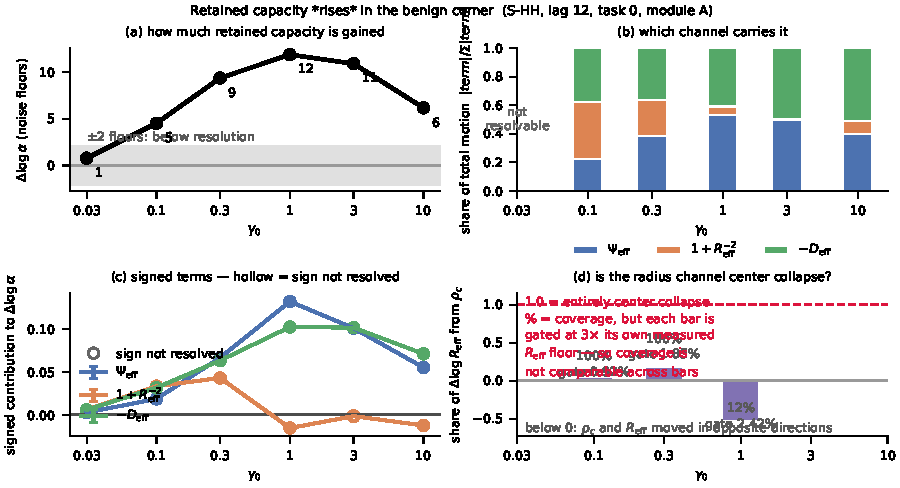
\includegraphics[width=\linewidth]
   {figures/fig2_gamma_sweep__S-HH__lag12__960arms__8dd793134c38.pdf}}
\end{figure}

\begin{figure}[t]
\floatconts
  {fig:lag4}
  {\caption{\textbf{The composition holds at a shorter lag.} Figure~\ref{fig:decomposition} at
   lag~4, task~0. Shares agree with lag~12 to within 0.032; magnitude changes by $1.27\times$.}}
  {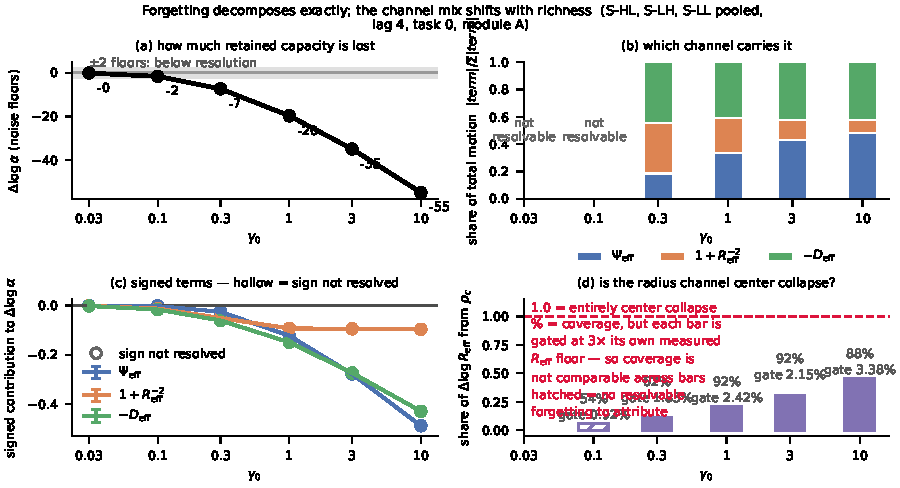
\includegraphics[width=\linewidth]
   {figures/fig2_gamma_sweep__forgetting__lag4__task0__960arms__8dd793134c38.pdf}}
\end{figure}

\begin{figure}[t]
\floatconts
  {fig:width}
  {\caption{\textbf{Width robustness, in the main figure's form.} Duplicate-stream matched
   subset (streams 0--1, seeds 0--1). The $\gamma_0=10$ contrast quoted in the text is genuine
   $n=40$ ($N=150$ vs $600$; magnitude varies by 0.62\%, utility share by 0.020).}}
  {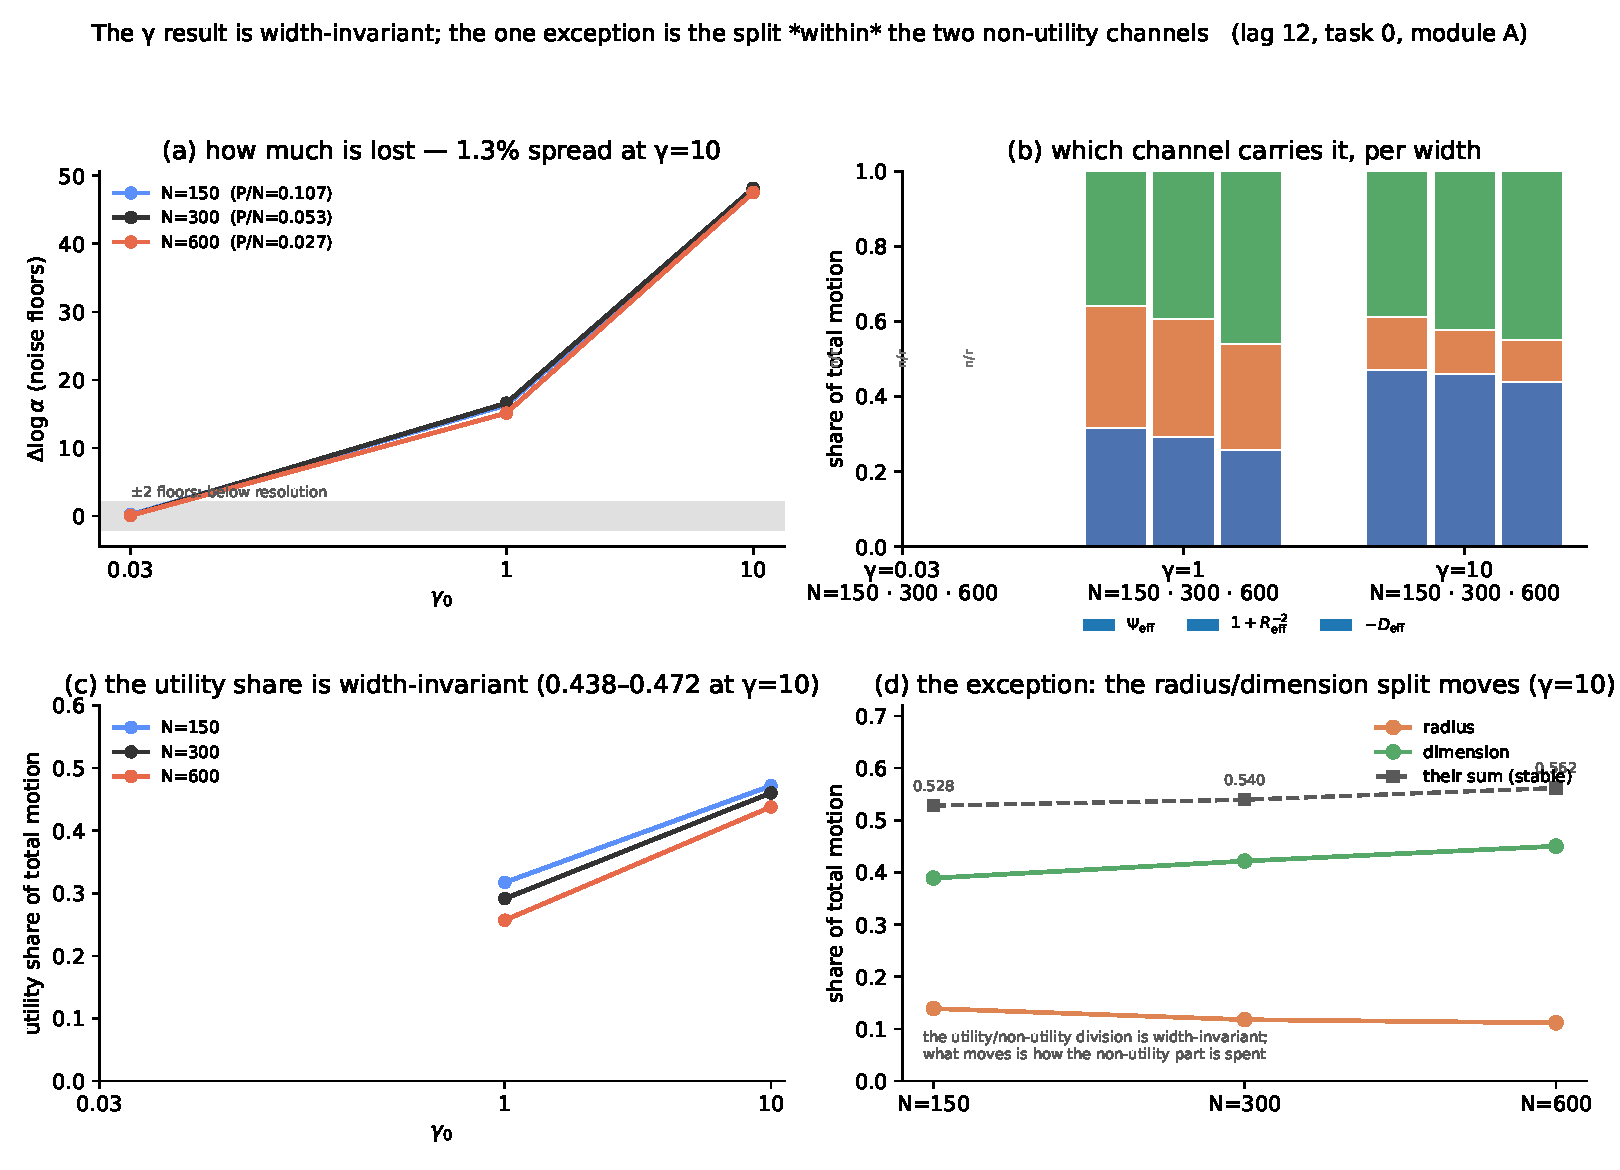
\includegraphics[width=\linewidth]
   {figures/fig_width_invariance__lag12__2f8b522a6423.pdf}}
\end{figure}

\begin{figure}[t]
\floatconts
  {fig:corners-gamma3}
  {\caption{\textbf{The corner structure at $\gamma_0=3$.} \texttt{S-HL} decorrelation absent
   ($+0.003$, 4 of 8 unique, $p=1.0$); present at $\gamma_0=10$ (8 of 8 unique). A $\gamma_0=5$
   probe is negative in four of eight arrangements, so the onset stays
   bracketed by the grid at a factor of 3.3.}}
  {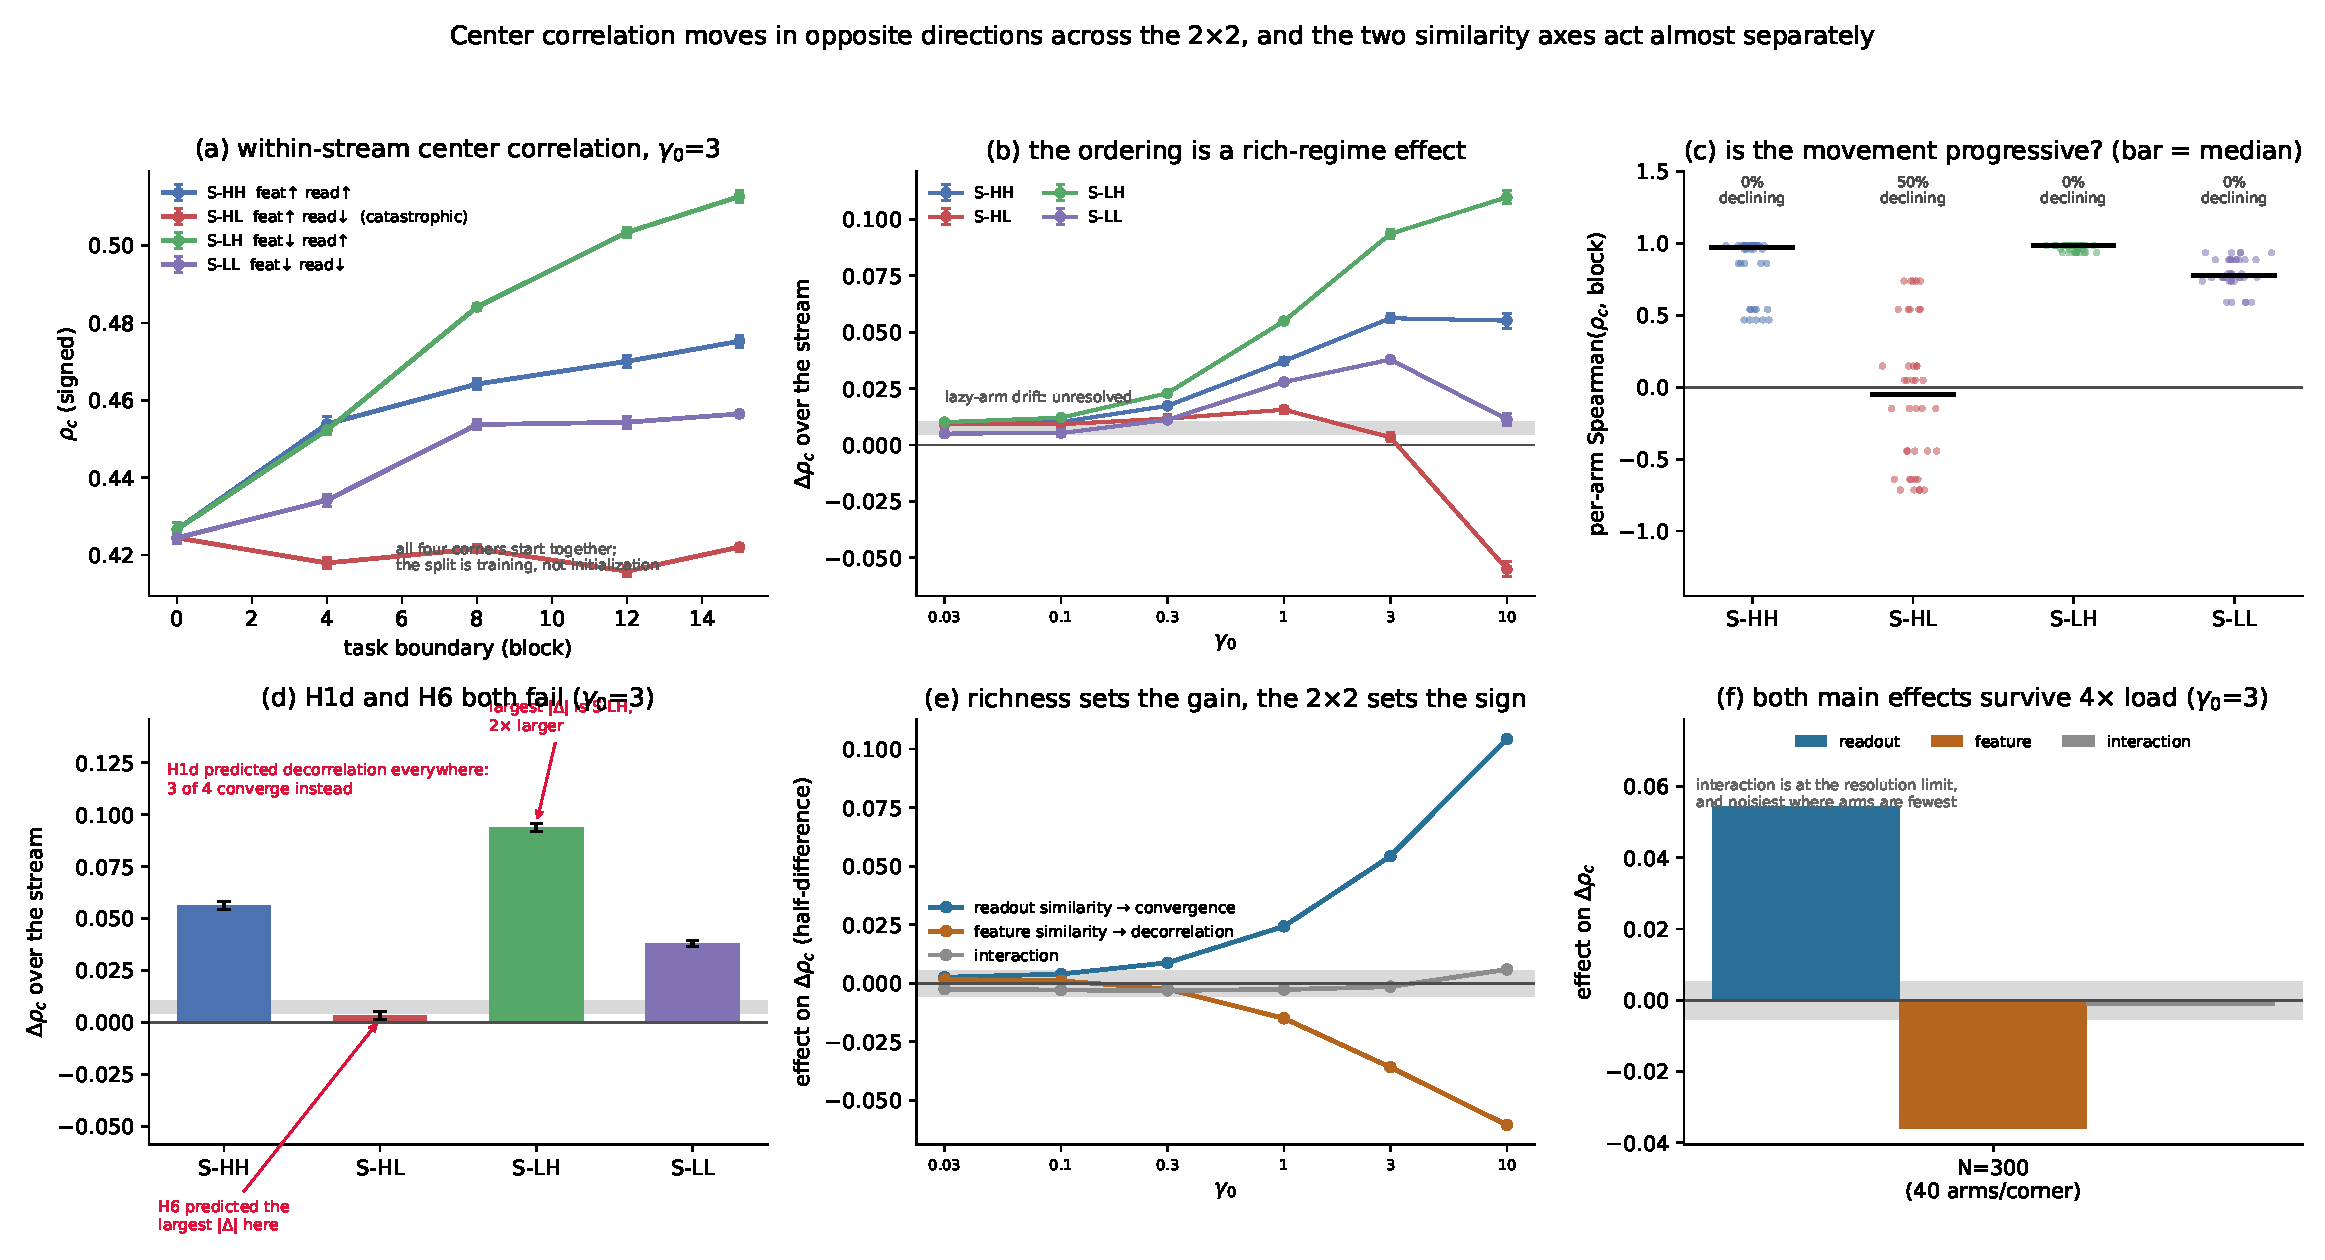
\includegraphics[width=\linewidth]
   {figures/fig4_corners_rho_c__gamma3__960arms__8dd793134c38.pdf}}
\end{figure}
 from the appendix, never from the body. Split out of figures.tex once the
% page count was measured: body plus all six floats is 5 pages against a limit of 4, and these four
% are what makes the difference. fig:benign is referenced from the caption of fig:decomposition, so
% dropping it entirely means editing that caption.


\begin{figure}[t]
\floatconts
  {fig:benign}
  {\caption{\textbf{The benign corner gains retained capacity.} The same decomposition as
   Figure~\ref{fig:decomposition}, for \texttt{S-HH} alone (8 unique seeds per $\gamma_0$; 40 files
   are copies). Largest at
   $\gamma_0=1$ (11.8 floors), 6.2 by $\gamma_0=10$. Radius term not resolved at $\gamma_0\geq 1$
   (1.9, 0.2, 1.1 floors) --- a bound under 2 floors, not a sign.}}
  {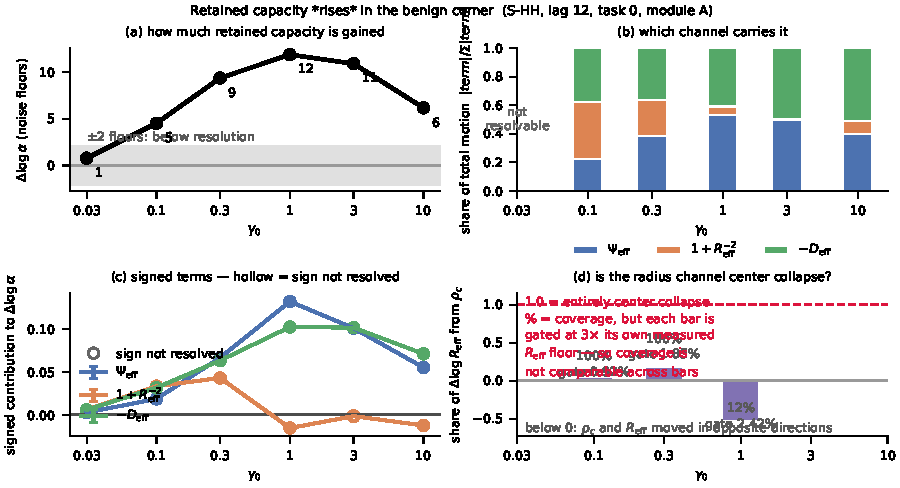
\includegraphics[width=\linewidth]
   {figures/fig2_gamma_sweep__S-HH__lag12__960arms__8dd793134c38.pdf}}
\end{figure}

\begin{figure}[t]
\floatconts
  {fig:lag4}
  {\caption{\textbf{The composition holds at a shorter lag.} Figure~\ref{fig:decomposition} at
   lag~4, task~0. Shares agree with lag~12 to within 0.032; magnitude changes by $1.27\times$.}}
  {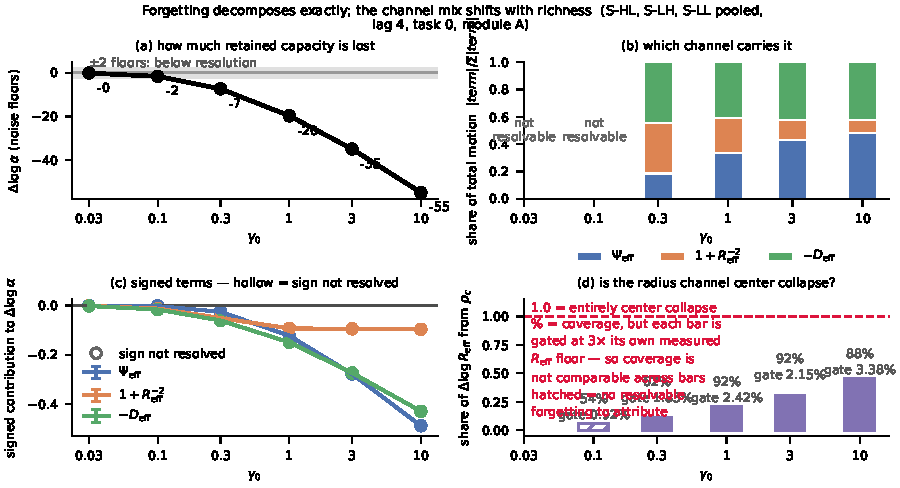
\includegraphics[width=\linewidth]
   {figures/fig2_gamma_sweep__forgetting__lag4__task0__960arms__8dd793134c38.pdf}}
\end{figure}

\begin{figure}[t]
\floatconts
  {fig:width}
  {\caption{\textbf{Width robustness, in the main figure's form.} Duplicate-stream matched
   subset (streams 0--1, seeds 0--1). The $\gamma_0=10$ contrast quoted in the text is genuine
   $n=40$ ($N=150$ vs $600$; magnitude varies by 0.62\%, utility share by 0.020).}}
  {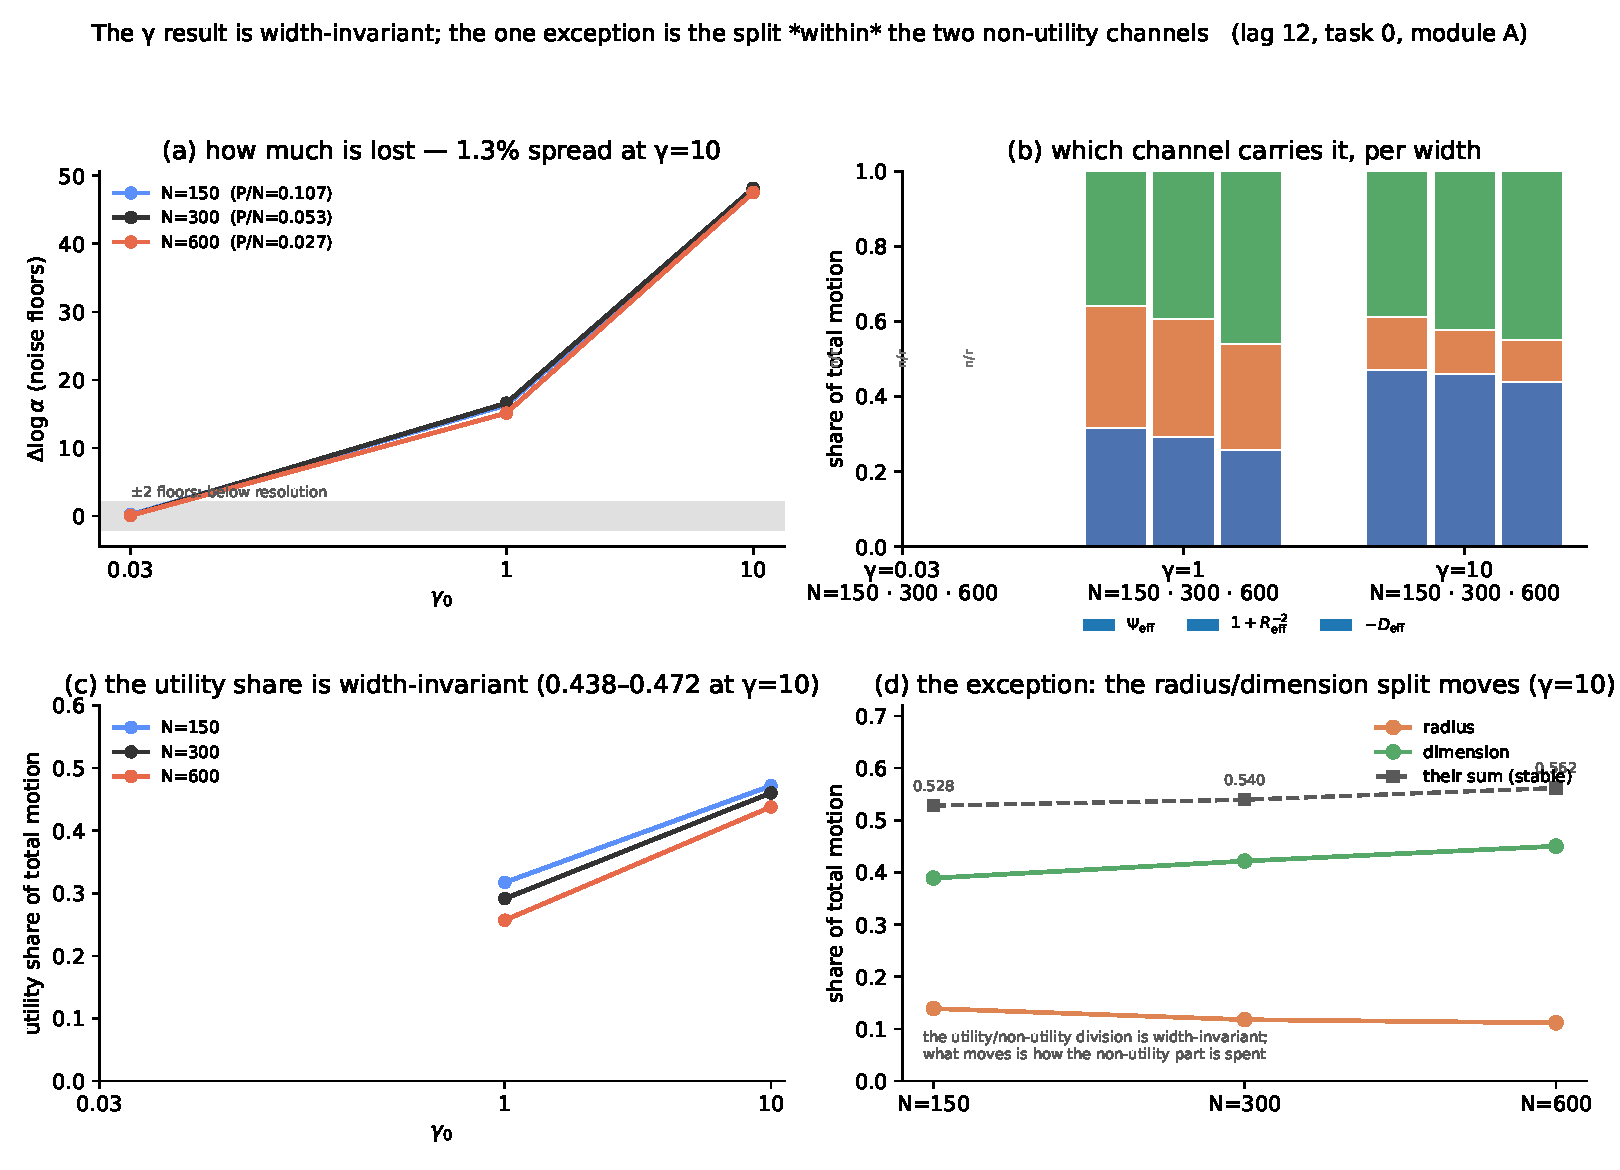
\includegraphics[width=\linewidth]
   {figures/fig_width_invariance__lag12__2f8b522a6423.pdf}}
\end{figure}

\begin{figure}[t]
\floatconts
  {fig:corners-gamma3}
  {\caption{\textbf{The corner structure at $\gamma_0=3$.} \texttt{S-HL} decorrelation absent
   ($+0.003$, 4 of 8 unique, $p=1.0$); present at $\gamma_0=10$ (8 of 8 unique). A $\gamma_0=5$
   probe is negative in four of eight arrangements, so the onset stays
   bracketed by the grid at a factor of 3.3.}}
  {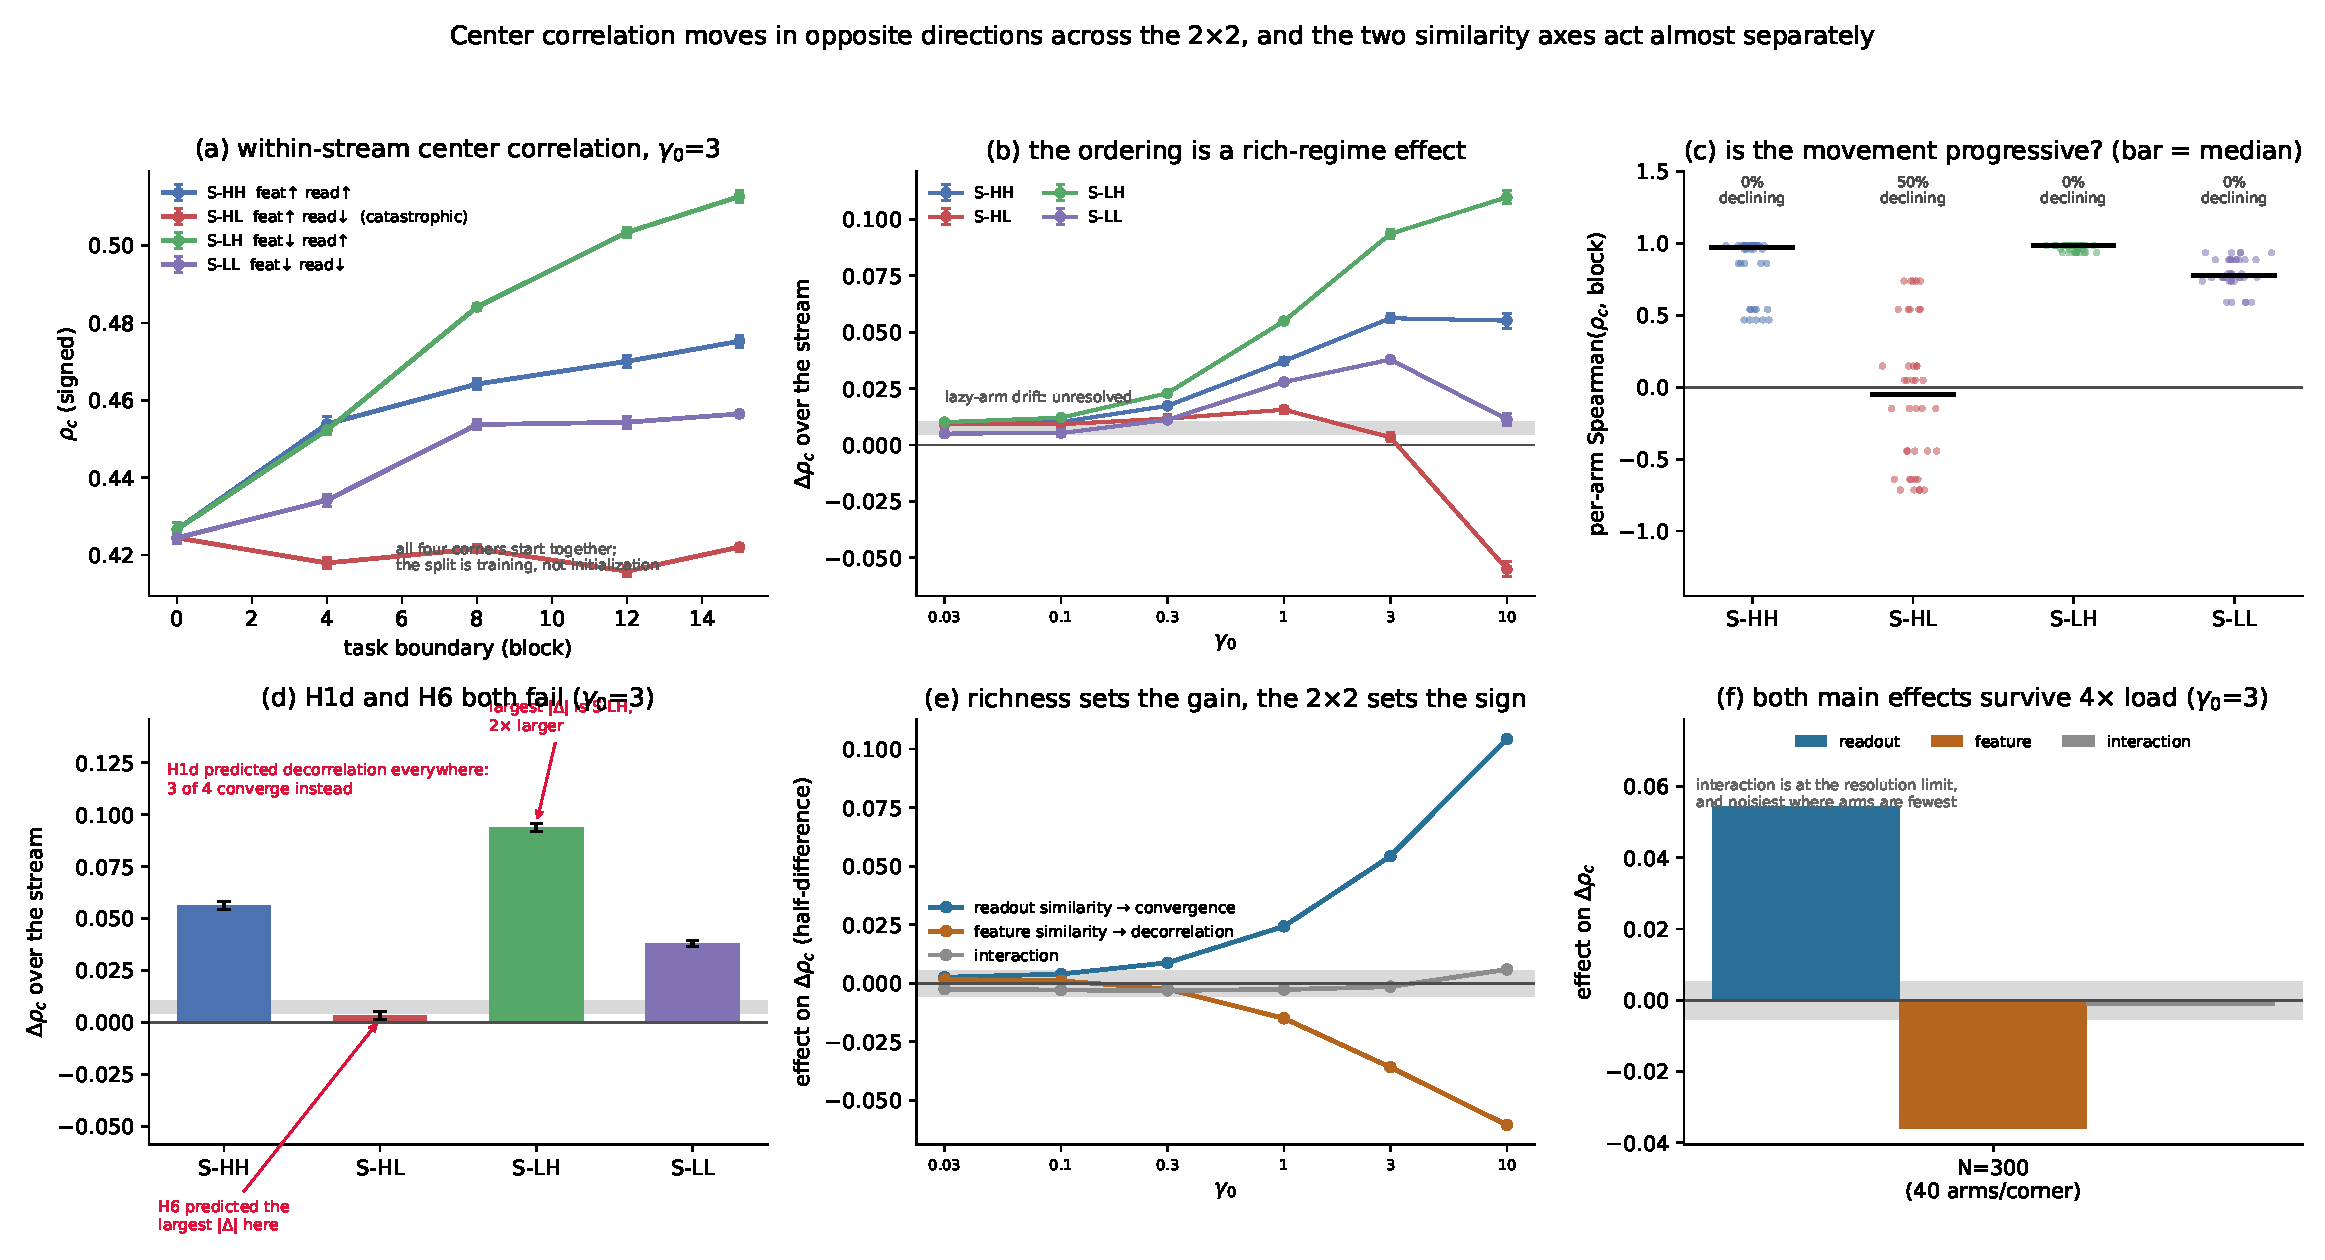
\includegraphics[width=\linewidth]
   {figures/fig4_corners_rho_c__gamma3__960arms__8dd793134c38.pdf}}
\end{figure}
 from the appendix, never from the body. Split out of figures.tex once the
% page count was measured: body plus all six floats is 5 pages against a limit of 4, and these four
% are what makes the difference. fig:benign is referenced from the caption of fig:decomposition, so
% dropping it entirely means editing that caption.


\begin{figure}[t]
\floatconts
  {fig:benign}
  {\caption{\textbf{The benign corner gains retained capacity.} The same decomposition as
   Figure~\ref{fig:decomposition}, for \texttt{S-HH} alone (8 unique seeds per $\gamma_0$; 40 files
   are copies). Largest at
   $\gamma_0=1$ (11.8 floors), 6.2 by $\gamma_0=10$. Radius term not resolved at $\gamma_0\geq 1$
   (1.9, 0.2, 1.1 floors) --- a bound under 2 floors, not a sign.}}
  {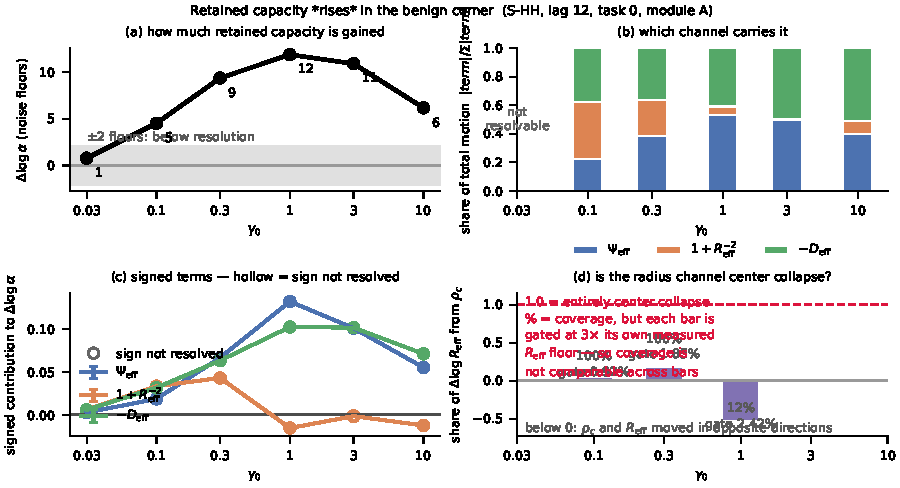
\includegraphics[width=\linewidth]
   {figures/fig2_gamma_sweep__S-HH__lag12__960arms__8dd793134c38.pdf}}
\end{figure}

\begin{figure}[t]
\floatconts
  {fig:lag4}
  {\caption{\textbf{The composition holds at a shorter lag.} Figure~\ref{fig:decomposition} at
   lag~4, task~0. Shares agree with lag~12 to within 0.032; magnitude changes by $1.27\times$.}}
  {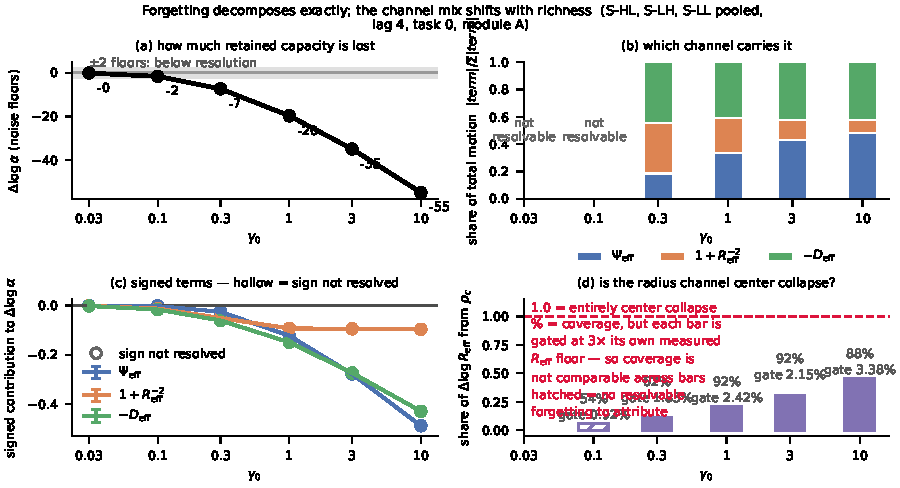
\includegraphics[width=\linewidth]
   {figures/fig2_gamma_sweep__forgetting__lag4__task0__960arms__8dd793134c38.pdf}}
\end{figure}

\begin{figure}[t]
\floatconts
  {fig:width}
  {\caption{\textbf{Width robustness, in the main figure's form.} Duplicate-stream matched
   subset (streams 0--1, seeds 0--1). The $\gamma_0=10$ contrast quoted in the text is genuine
   $n=40$ ($N=150$ vs $600$; magnitude varies by 0.62\%, utility share by 0.020).}}
  {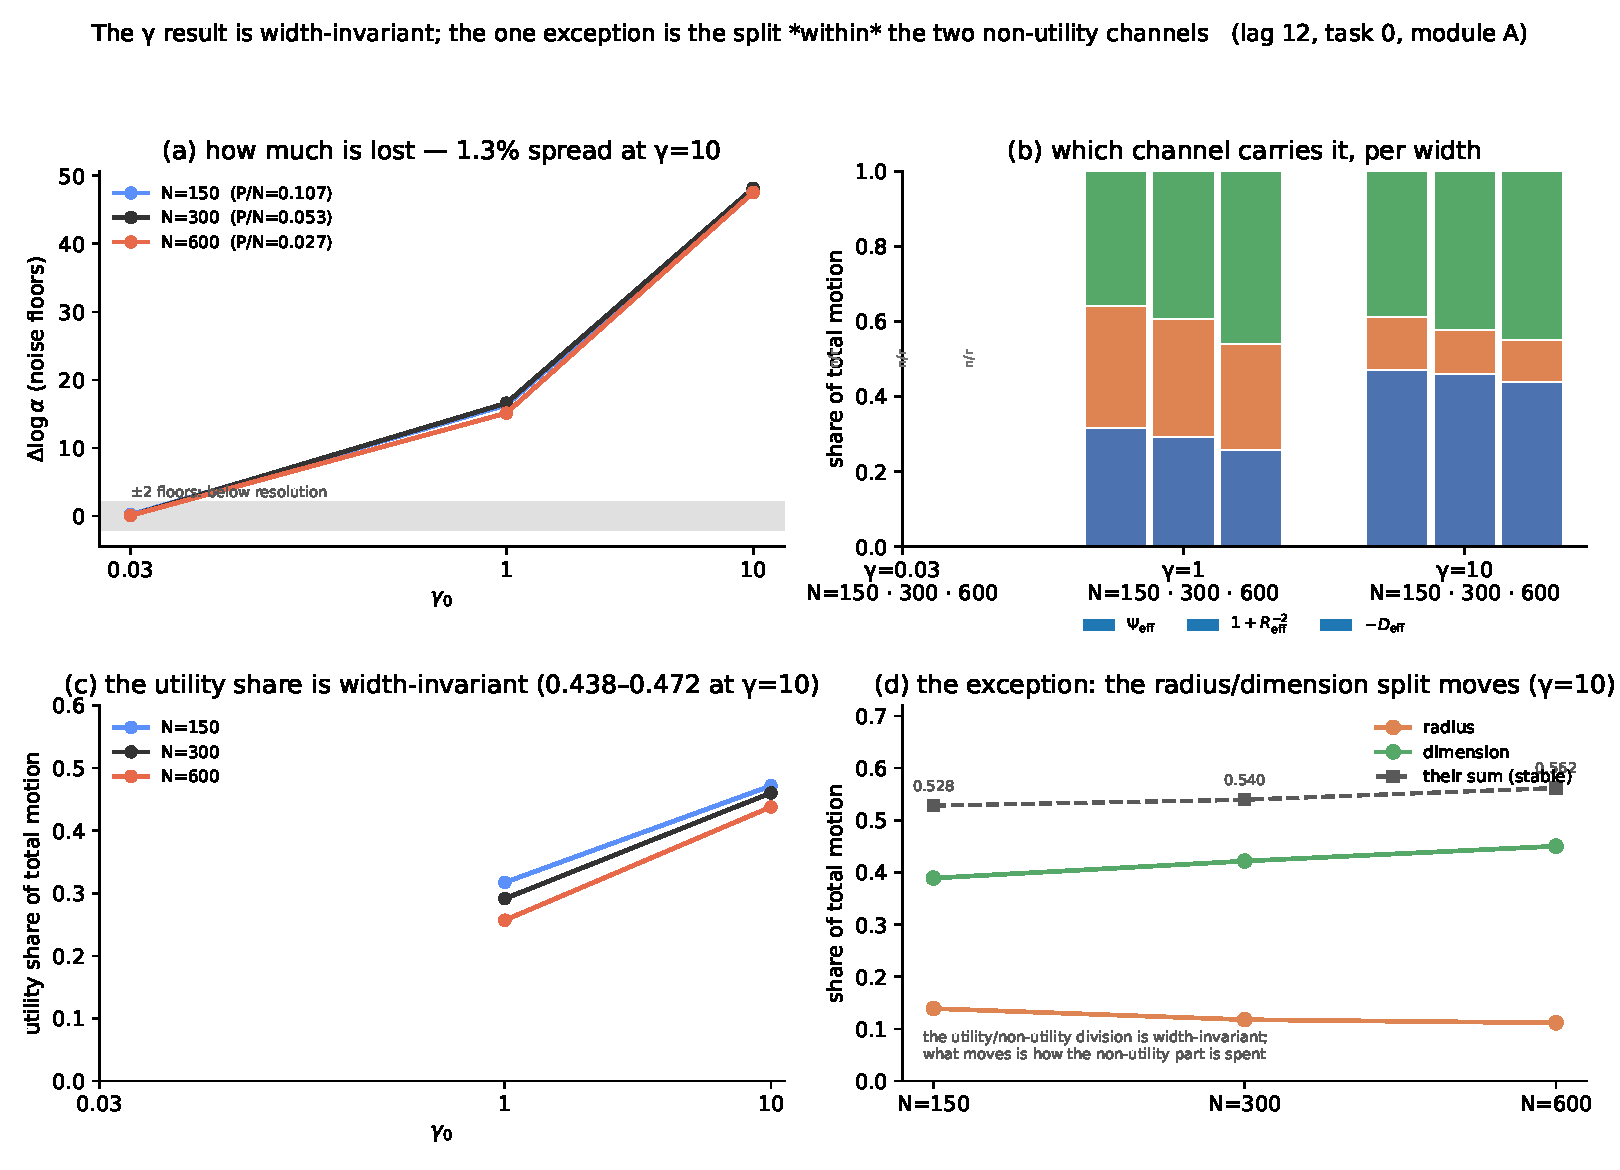
\includegraphics[width=\linewidth]
   {figures/fig_width_invariance__lag12__2f8b522a6423.pdf}}
\end{figure}

\begin{figure}[t]
\floatconts
  {fig:corners-gamma3}
  {\caption{\textbf{The corner structure at $\gamma_0=3$.} \texttt{S-HL} decorrelation absent
   ($+0.003$, 4 of 8 unique, $p=1.0$); present at $\gamma_0=10$ (8 of 8 unique). A $\gamma_0=5$
   probe is negative in four of eight arrangements, so the onset stays
   bracketed by the grid at a factor of 3.3.}}
  {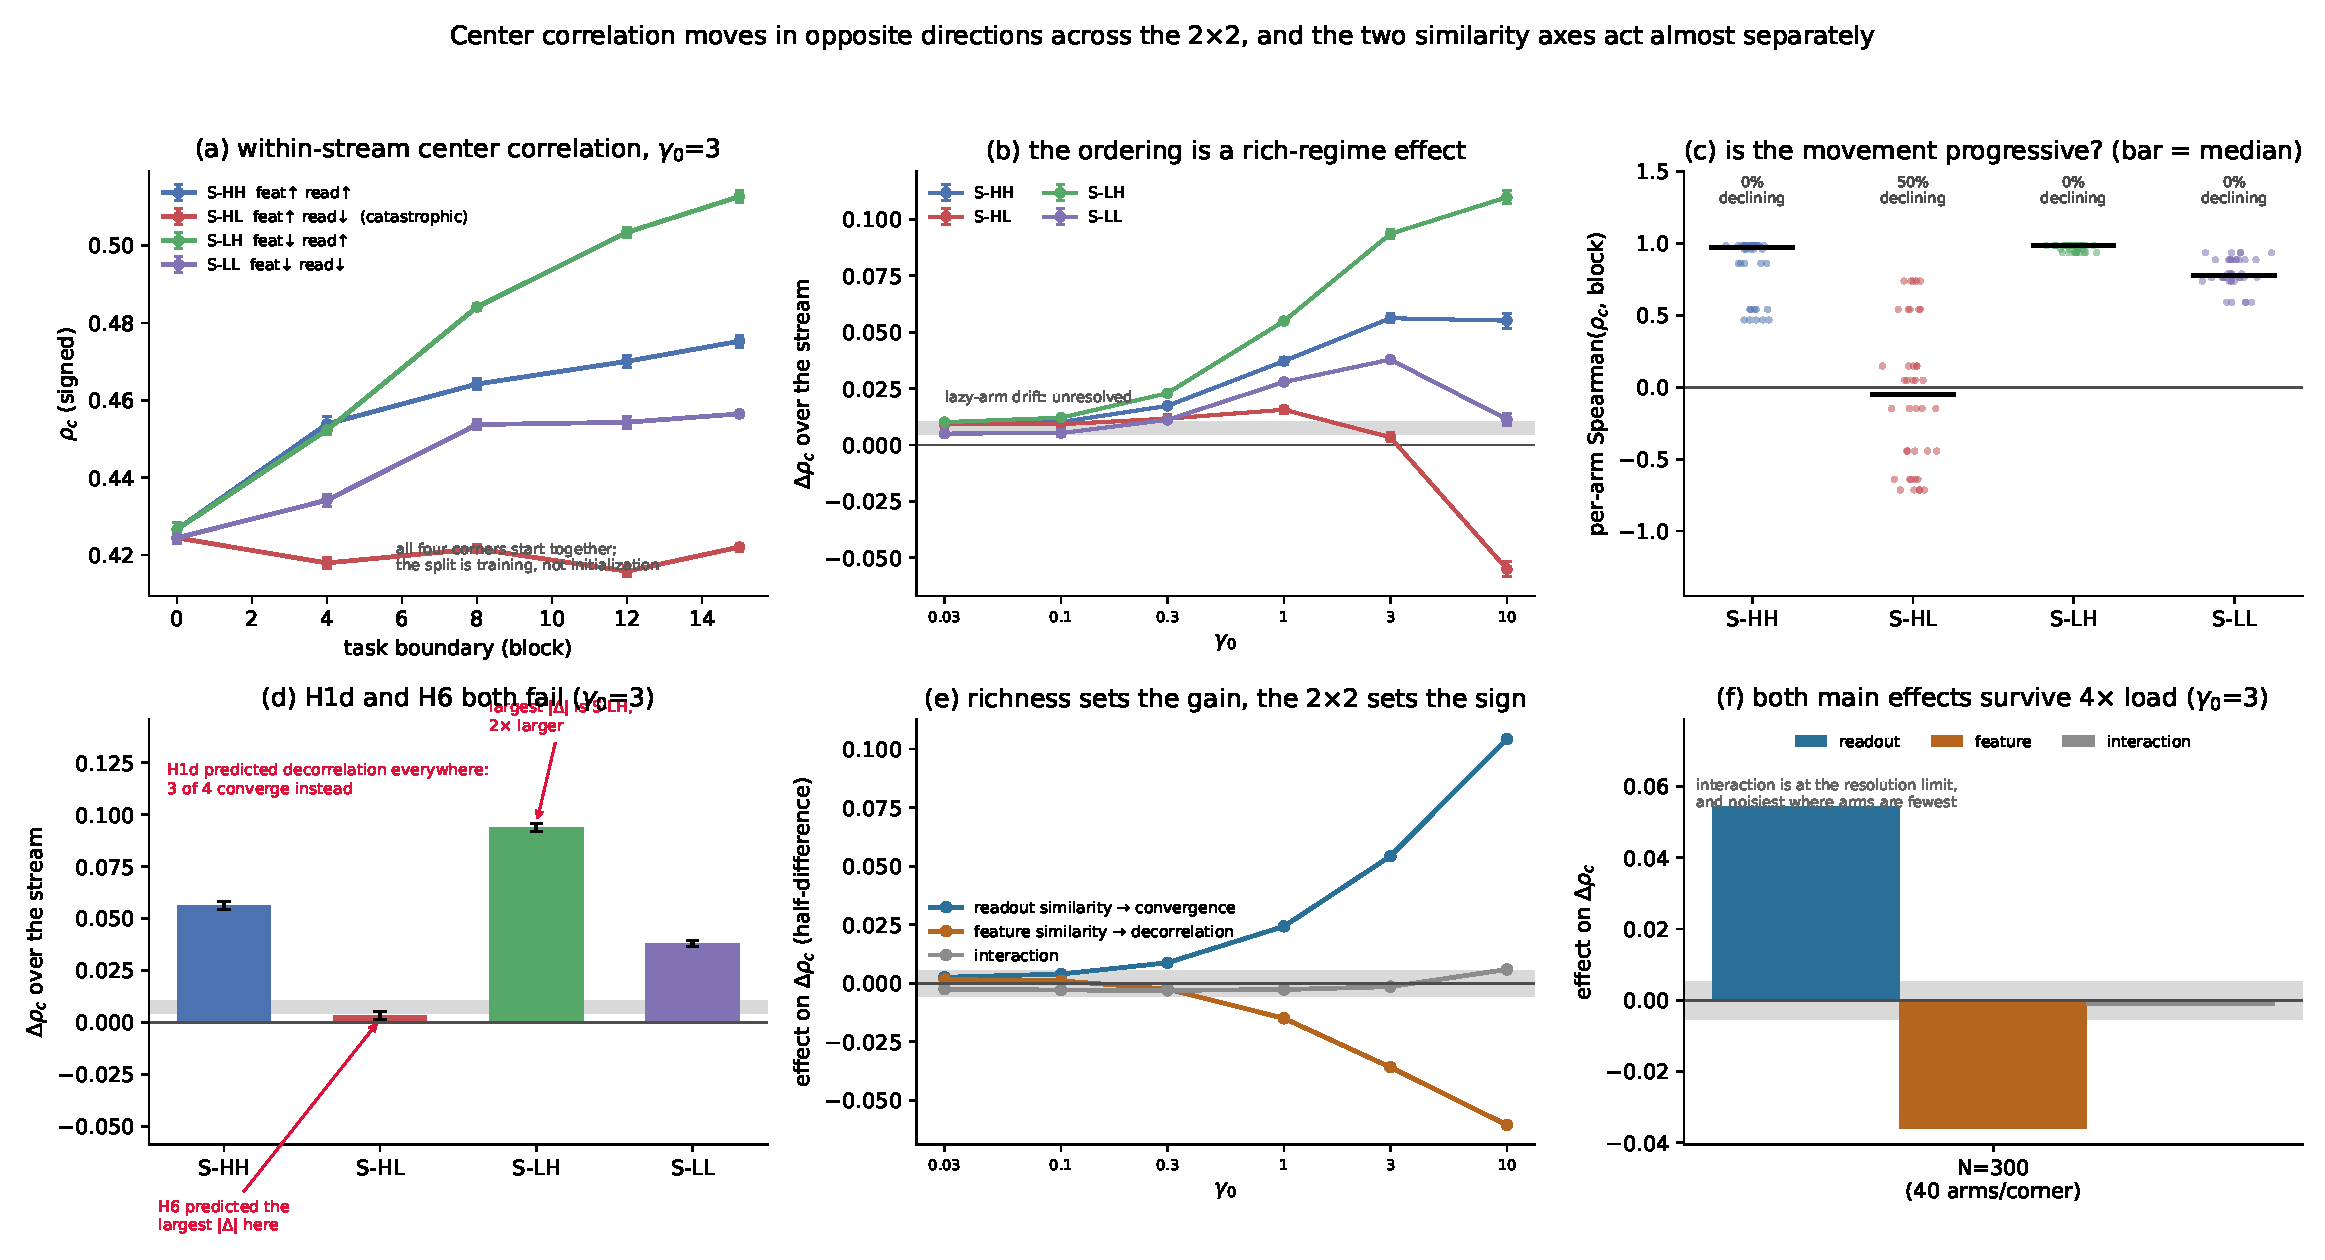
\includegraphics[width=\linewidth]
   {figures/fig4_corners_rho_c__gamma3__960arms__8dd793134c38.pdf}}
\end{figure}
 from the appendix, never from the body. Split out of figures.tex once the
% page count was measured: body plus all six floats is 5 pages against a limit of 4, and these four
% are what makes the difference. fig:benign is referenced from the caption of fig:decomposition, so
% dropping it entirely means editing that caption.


\begin{figure}[t]
\floatconts
  {fig:benign}
  {\caption{\textbf{The benign corner gains retained capacity.} The same decomposition as
   Figure~\ref{fig:decomposition}, for \texttt{S-HH} alone (8 unique seeds per $\gamma_0$; 40 files
   are copies). Largest at
   $\gamma_0=1$ (11.8 floors), 6.2 by $\gamma_0=10$. Radius term not resolved at $\gamma_0\geq 1$
   (1.9, 0.2, 1.1 floors) --- a bound under 2 floors, not a sign.}}
  {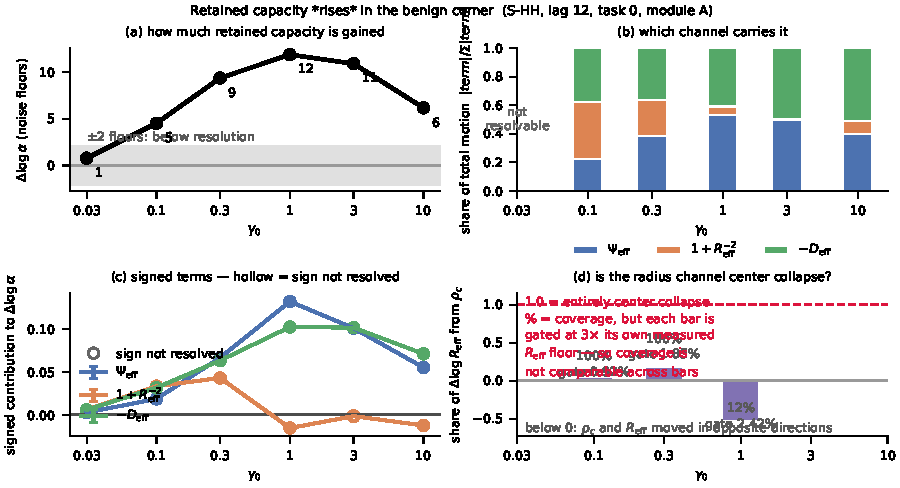
\includegraphics[width=\linewidth]
   {figures/fig2_gamma_sweep__S-HH__lag12__960arms__8dd793134c38.pdf}}
\end{figure}

\begin{figure}[t]
\floatconts
  {fig:lag4}
  {\caption{\textbf{The composition holds at a shorter lag.} Figure~\ref{fig:decomposition} at
   lag~4, task~0. Shares agree with lag~12 to within 0.032; magnitude changes by $1.27\times$.}}
  {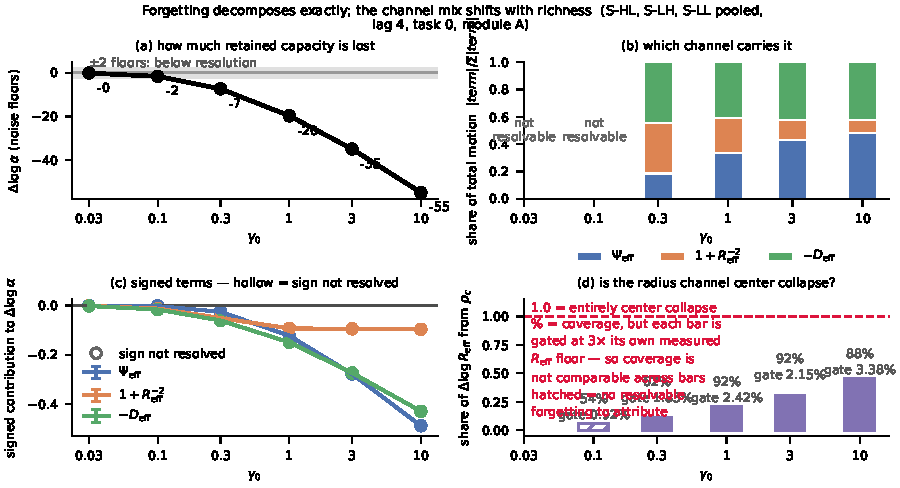
\includegraphics[width=\linewidth]
   {figures/fig2_gamma_sweep__forgetting__lag4__task0__960arms__8dd793134c38.pdf}}
\end{figure}

\begin{figure}[t]
\floatconts
  {fig:width}
  {\caption{\textbf{Width robustness, in the main figure's form.} Duplicate-stream matched
   subset (streams 0--1, seeds 0--1). The $\gamma_0=10$ contrast quoted in the text is genuine
   $n=40$ ($N=150$ vs $600$; magnitude varies by 0.62\%, utility share by 0.020).}}
  {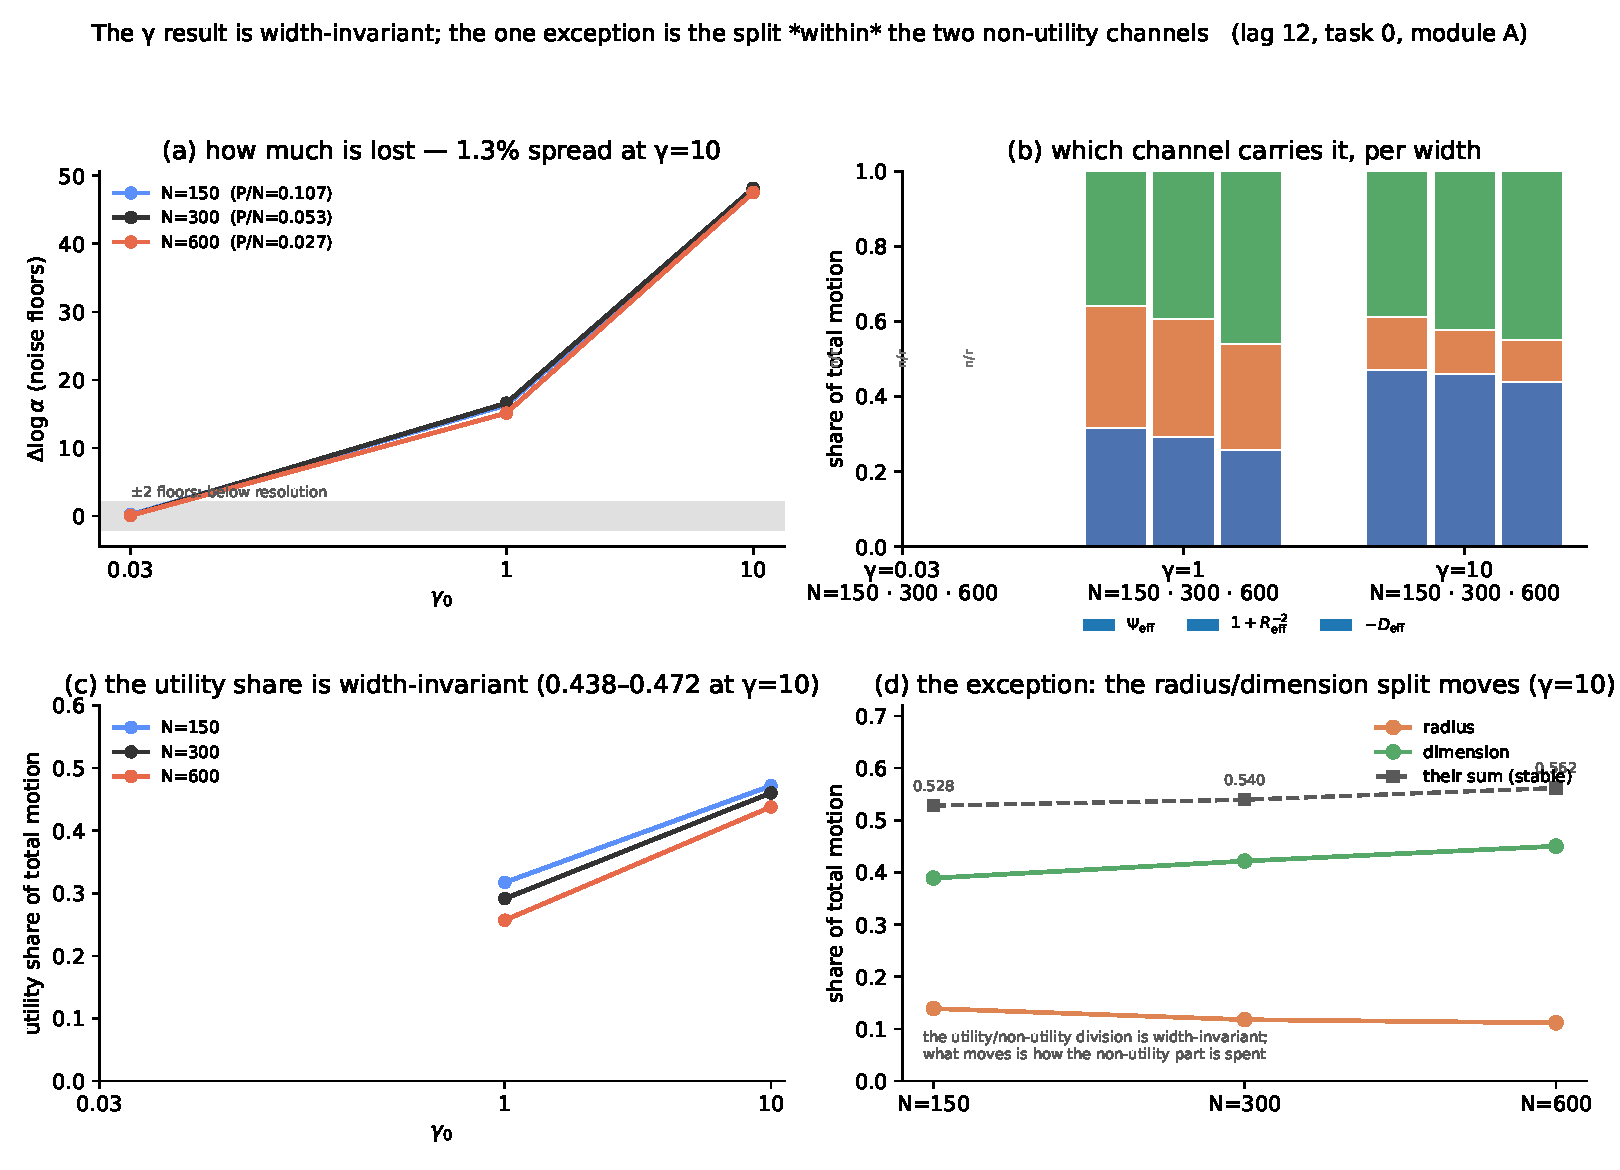
\includegraphics[width=\linewidth]
   {figures/fig_width_invariance__lag12__2f8b522a6423.pdf}}
\end{figure}

\begin{figure}[t]
\floatconts
  {fig:corners-gamma3}
  {\caption{\textbf{The corner structure at $\gamma_0=3$.} \texttt{S-HL} decorrelation absent
   ($+0.003$, 4 of 8 unique, $p=1.0$); present at $\gamma_0=10$ (8 of 8 unique). A $\gamma_0=5$
   probe is negative in four of eight arrangements, so the onset stays
   bracketed by the grid at a factor of 3.3.}}
  {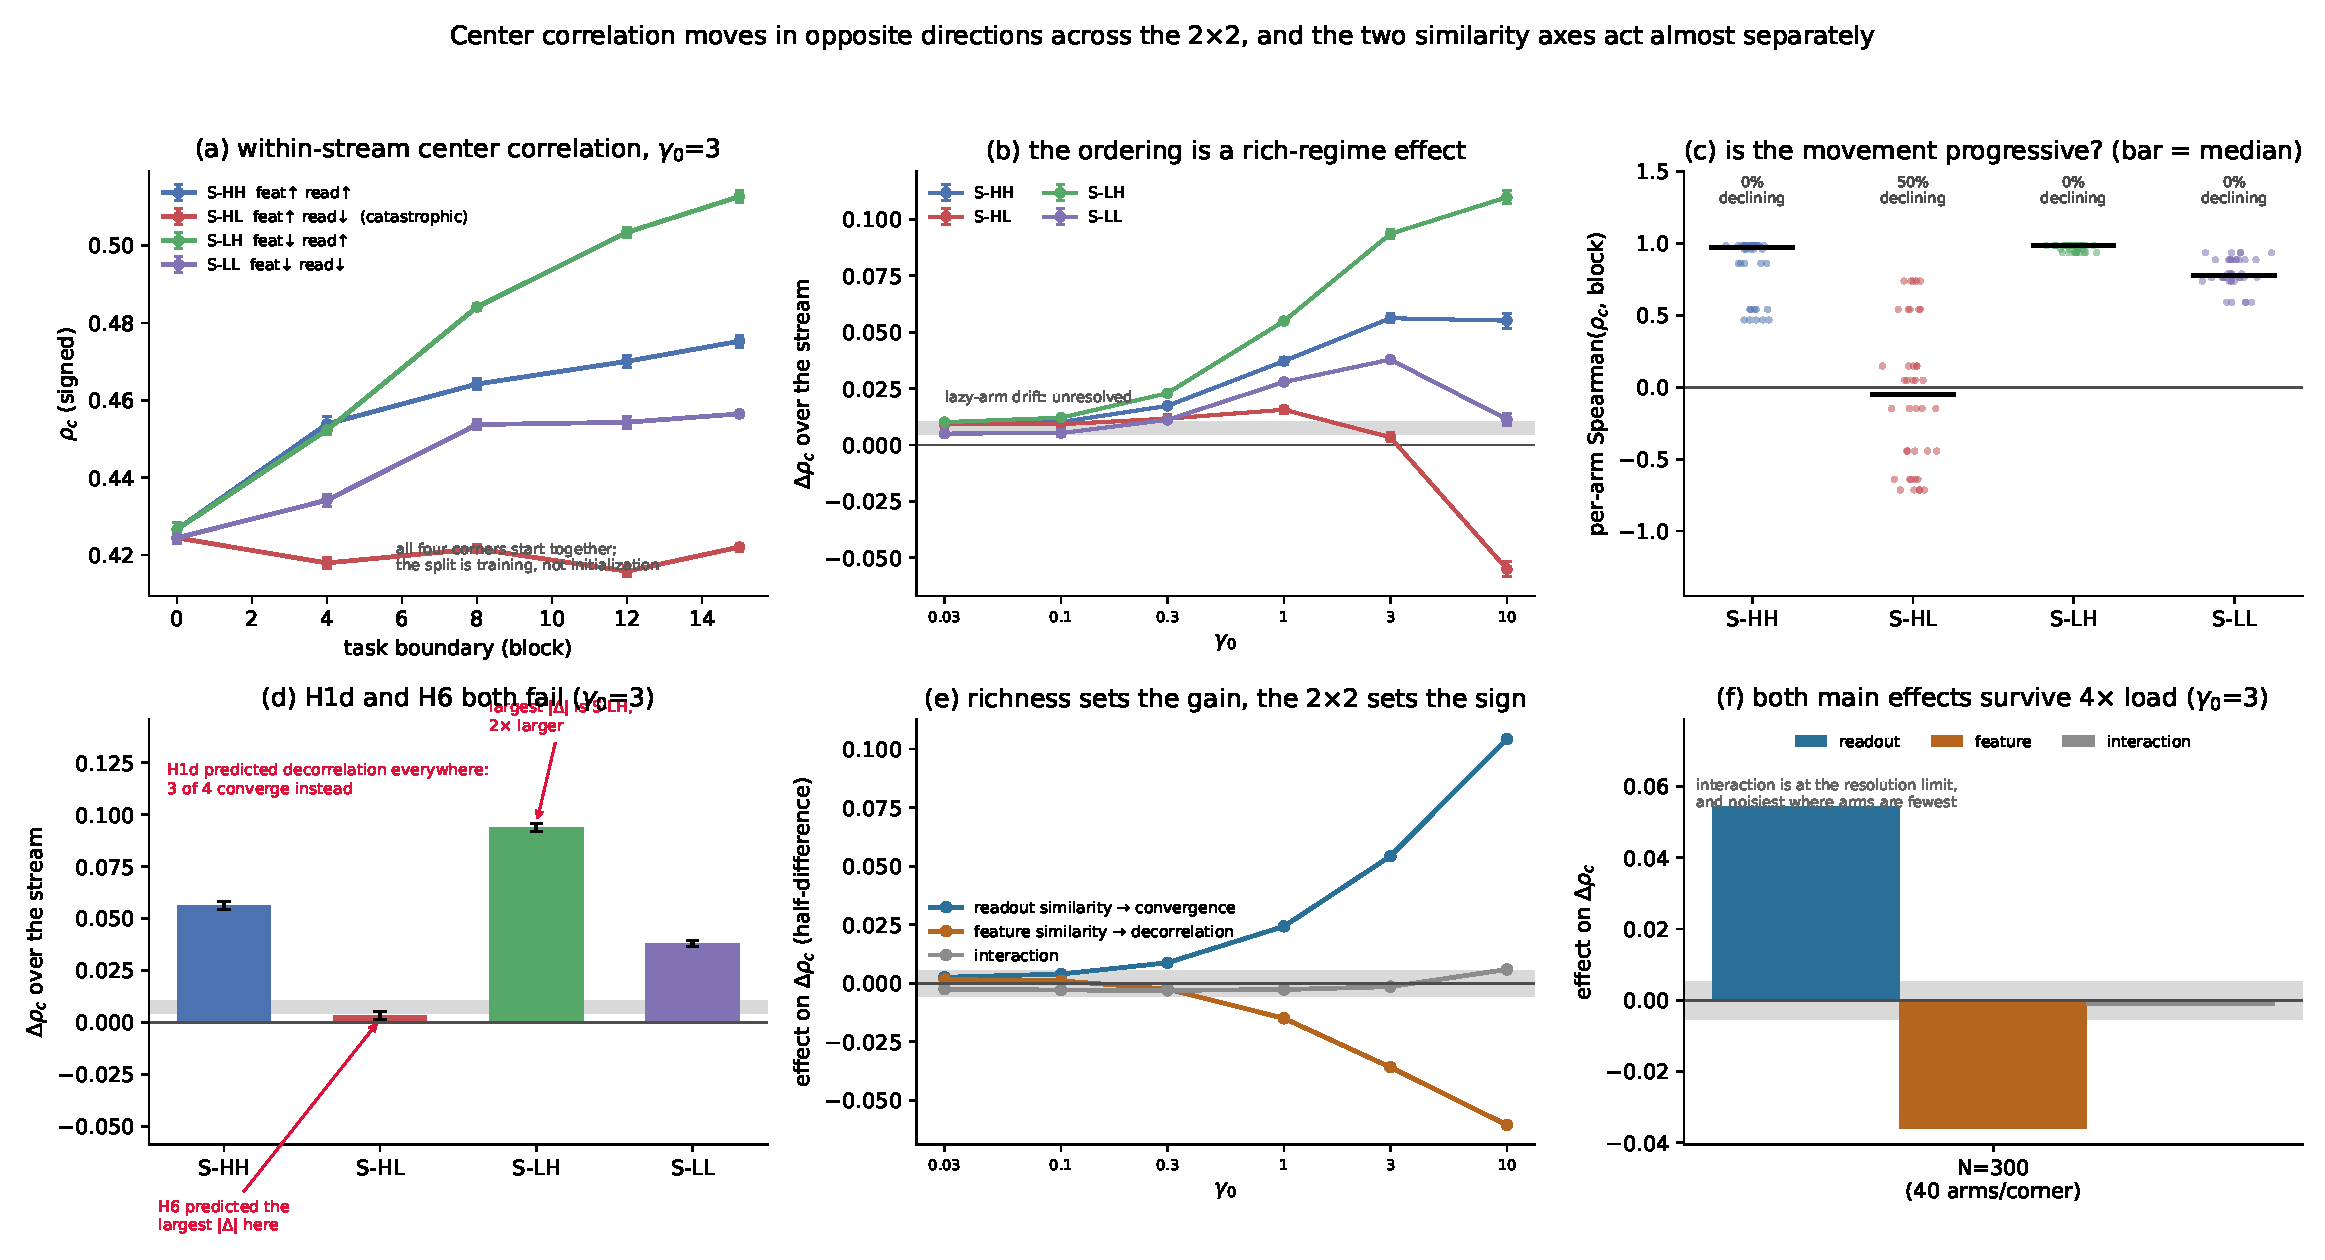
\includegraphics[width=\linewidth]
   {figures/fig4_corners_rho_c__gamma3__960arms__8dd793134c38.pdf}}
\end{figure}
